\documentclass[12pt, a4paper, oneside]{ctexart}
\usepackage{amsmath, amsthm, amssymb, bm, color, graphicx, geometry, mathrsfs,extarrows, braket, booktabs, array}
\usepackage[colorlinks,linkcolor=red,anchorcolor=blue,citecolor=blue,urlcolor=blue,menucolor=black]{hyperref}
%%%% 设置中文字体 %%%%
\setCJKmainfont{方正新书宋_GBK.ttf}[ BoldFont = 方正小标宋_GBK, ItalicFont = 方正楷体_GBK]
%%%% 设置英文字体 %%%%
\setmainfont{Times New Roman}
\setsansfont{Calibri}
\setmonofont{Consolas}

\linespread{1.4}
%\geometry{left=2.54cm,right=2.54cm,top=3.18cm,bottom=3.18cm}
\geometry{left=1.84cm,right=1.84cm,top=2.18cm,bottom=2.18cm}
\newcounter{problem}  % 问题序号计数器
\newenvironment{problem}{\stepcounter{problem}\par\noindent\textbf{题目\arabic{problem}. }}{\smallskip\par}
\newenvironment{solution}{\par\noindent\textbf{解答. }}{\smallskip\par}
\newenvironment{note}{\par\noindent\textbf{注记. }}{\smallskip\par}

\usepackage{minted}
\renewcommand{\theFancyVerbLine}{
    \sffamily\textcolor[rgb]{0.5,0.5,0.5}{\scriptsize\arabic{FancyVerbLine}}} % 修改代码前序号大小
\newmintinline{python}{linenos, breaklines, frame=lines, python3}  % 使用\pythoninline{代码}
\newmintinline{cpp}{linenos, breaklines, frame=lines}  % 使用\c++inline{代码}
\newminted{python}{linenos, breaklines, frame=lines, python3}  % 使用\begin{pythoncode}代码\end{pythoncode}
\newminted{cpp}{linenos, breaklines, frame=lines}  % 使用\begin{pythoncode}代码\end{pythoncode}
\newmintedfile{python}{linenos, breaklines, frame=lines, python3}  % 使用\pythonfile{代码地址}

%%%% 图片相对路径 %%%%
\graphicspath{{figure/}} % 当前目录下的figure文件夹, {../figure/}则是父目录的figure文件夹

\everymath{\displaystyle} % 默认全部行间公式
\DeclareMathOperator*\uplim{\overline{lim}} % 定义上极限 \uplim_{}
\DeclareMathOperator*\lowlim{\underline{lim}} % 定义下极限 \lowlim_{}
\let\leq=\leqslant % 将全部leq变为leqslant
\let\geq=\geqslant % geq同理

%%%% 一些宏定义 %%%%
\def\bd{\boldsymbol}        % 加粗(向量) boldsymbol
\def\disp{\displaystyle}    % 使用行间公式 displaystyle(默认)
\def\tsty{\textstyle}       % 使用行内公式 textstyle
\def\sign{\text{sign}}      % sign function
\def\wtd{\widetilde}        % 宽波浪线 widetilde
\def\R{\mathbb{R}}          % Real number
\def\N{\mathbb{N}}          % Natural number
\def\Z{\mathbb{Z}}          % Integer number
\def\Q{\mathbb{Q}}          % Rational number
\def\C{\mathbb{C}}          % Complex number
\def\d{\mathrm{d}}          % differential operator
\def\e{\mathrm{e}}          % Euler's number
\def\i{\mathrm{i}}          % imaginary number
\def\re{\mathrm{Re}}        % Real part
\def\im{\mathrm{Im}}        % Imaginary part
\def\res{\mathrm{Res}}      % Residue
\def\L{\mathcal{L}}         % Loss function
\def\wdh{\widehat}          % 宽帽子 widehat
\def\ol{\overline}          % 上横线 overline
\def\ul{\underline}         % 下横线 underline
\def\add{\vspace{1ex}}      % 增加行间距
\def\del{\vspace{-3.5ex}}   % 减少行间距

%%%% 定理类环境的定义 %%%%
\newtheorem{theorem}{定理}

%%%% 基本信息 %%%%
\newcommand{\RQ}{\today} % 日期
\newcommand{\km}{算法设计与分析} % 科目
\newcommand{\bj}{强基数学002} % 班级
\newcommand{\xm}{吴天阳} % 姓名
\newcommand{\xh}{2204210460} % 学号

\begin{document}

%\pagestyle{empty}
\pagestyle{plain}
\vspace*{-15ex}
\centerline{\begin{tabular}{*5{c}}
    \parbox[t]{0.25\linewidth}{\begin{center}\textbf{日期}\\ \large \textcolor{blue}{\RQ}\end{center}} 
    & \parbox[t]{0.25\linewidth}{\begin{center}\textbf{科目}\\ \large \textcolor{blue}{\km}\end{center}}
    & \parbox[t]{0.2\linewidth}{\begin{center}\textbf{班级}\\ \large \textcolor{blue}{\bj}\end{center}}
    & \parbox[t]{0.1\linewidth}{\begin{center}\textbf{姓名}\\ \large \textcolor{blue}{\xm}\end{center}}
    & \parbox[t]{0.15\linewidth}{\begin{center}\textbf{学号}\\ \large \textcolor{blue}{\xh}\end{center}} \\ \hline
\end{tabular}}
\begin{center}
    \zihao{3}\textbf{第一次作业}
\end{center}\vspace{-0.2cm}
\begin{problem}
    (1) 假设某算法在输入规模为$n$时的计算时间为$T(n)=3\times 2^n$.在某台计算机上实现并完成该算法的时间为$t$秒.现有另一台计算机,其运行速度为第一台的$64$倍,那么在这台新机器上用同一算法在t秒内能解输入规模为多大的问题?

    (2)若上述算法的计算时间改进为$T(n)=n^2$,其余条件不变,则在新机器上用$t$秒时间能解输入规模为多大的问题?

    (3)若上述算法的计算时间进一步改进为$T(n)=8$,其余条件不变,那么在新机器上用$t$秒时间能解输入规模为多大的问题?
\end{problem}
\begin{solution}
    (1) $t = 3\times 2^n$,则$64t = 64\times 3\times 2^n = 3\times 2^{n+5}$,所以新机器可解决$n+5$规模的数据.

    (2) $t = n^2$,则$64t = (5n)^5$,所以新机器可解决$5n$规模的数据.

    (3) $t = 8n$,则$64t = 8\times(64n)$,所以新机器可解决$64n$规模的数据.
\end{solution}
\begin{problem}
    证明:如果一个算法在平均情况下的计算时间复杂性为$\theta(f(n))$,则该算法在最坏情况下所需的计算时间为$\Omega(f(n))$。
\end{problem}
\begin{proof}设$D_N$为规模为$N$的数据集.
    $T_{arg}(N) = \sum_{I\in D}P(I)f(I)\leq \max_{I\in D_N}f(I)\sum_{I\in D_N}P(I) = \max_{I\in D_N}f(I)$,所以该算法计算时间的上界为$\Omega(f(n))$.
\end{proof}

\begin{problem}
已知计算函数$F(n)$($n$为非负整数)的算法如下:
\begin{cppcode}
int F(int n){
    if (n==0) return 1;
    int s=0;
    for (int i=0;i<n;i++) s=s+F(i);
    return s+1;
}
\end{cppcode}
上述算法在计算$F(n)$的过程中,调用执行$F(0)$的次数是多少?
给出函数$F(n)$的非递归算术表达式;
分析上述算法的时间复杂度(给出复杂度的递归表达式,并求解)。
\end{problem}
\begin{solution}
    $F(n)$调用$F(0)$的次数为$2^{n-1}$. 非递归算术表达式为$F(n) = 2^n$. 时间复杂度的递归表达式为$T(n) =\sum_{k=0}^{n-1}T(k)$,令$T(0)=1$,则通过数学归纳法可知,$T(n) = 2^{n-1},\ n\geq 1$. 下面使用归纳法进行证明,$T(1) = T(0) = 1$,假设$n-1$时原命题成立,由命题假设可知
    \begin{equation*}
        F(n) = \sum_{k=1}^{n-1}2^{k-1}+1 = \frac{1-2^{n-1}}{1-2}+1 = 2^{n-1}.
    \end{equation*}
    故原命题得证.
\end{solution}

% 正文部分

% 下面给一些功能的写法
\iffalse
% 图片模板
\centerline{
    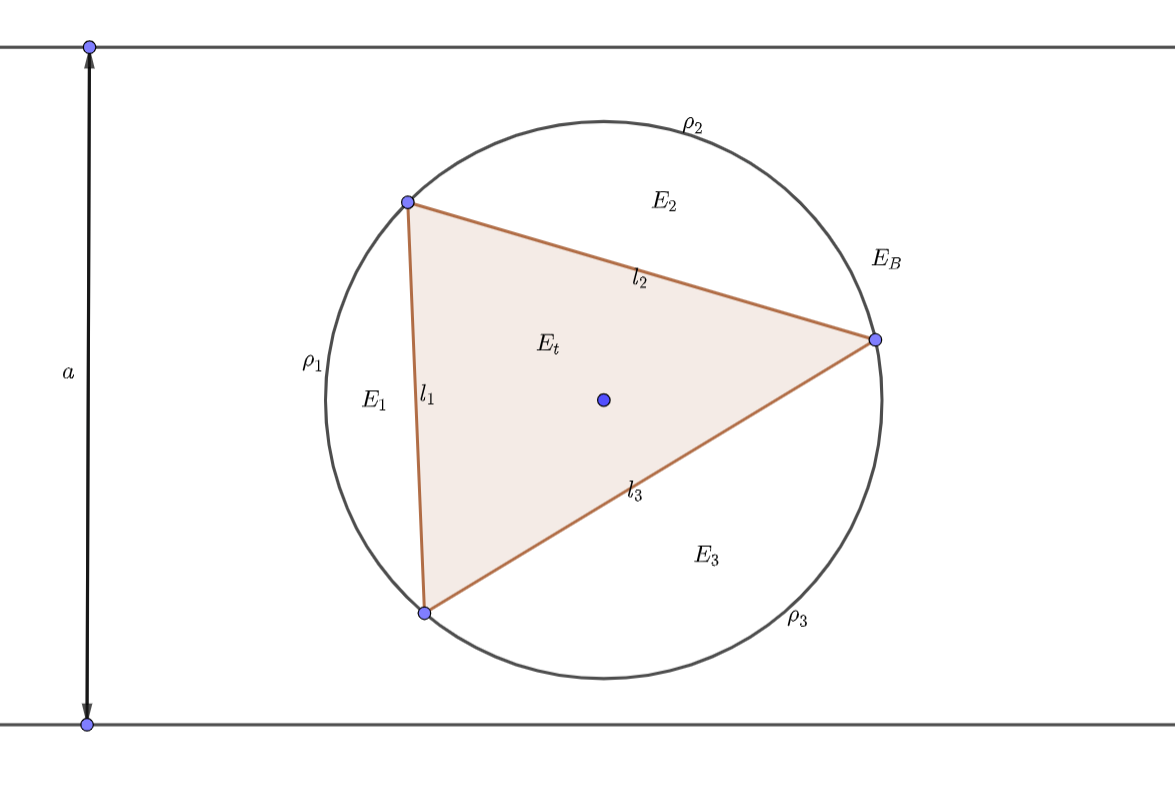
\includegraphics[width=0.8\textwidth]{figure.png}
}
% 表格模板
\renewcommand\arraystretch{0.8} % 设置表格高度为原来的0.8倍
\begin{table}[!htbp] % table标准
    \centering % 表格居中
    \begin{tabular}{p{1cm}<{\centering}p{1cm}<{\centering}p{3cm}<{\centering}p{5cm}<{\centering}} % 设置表格宽度
    %\begin{tabular}{cccc}
        \toprule
        $x_i$ & $f[x_1]$ & $f[x_i,x_{i+1}]$ & $f[x_i,x_{i+1},x_{i+2}]$ \\
        \midrule
        $x_0$ & $f(x_0)$ &                  &                          \\
        $x_0$ & $f(x_0)$ & $f'(x_0)$        &                          \\
        $x_0$ & $f(x_1)$ & $\frac{f(x_1)-f(x_0)}{x_1-x_0}$ & $\frac{f(x_1)-f(x_0)}{(x_1-x_0)^2}-\frac{f'(x_0)}{x_1-x_0}$\\
        \bottomrule
    \end{tabular}
\end{table}

\def\Log{\text{Log}} % 一个简单的宏定义
$\Log$ % 调用方法
\fi

\end{document}